
\section{Theory}
\label{sec:theory}
We describe the setup for Craig interpolation in the ring
$R=\Fq[x_1,\dots,x_n]$. Partition the variables $\{x_1,\dots,x_n\}$
into disjoint subsets $A, B, C$. We are given two ideals $J_A \subset
\Fq[A,C], J_B \subset \Fq[B,C]$ such that the $C$-variables are common
to the generators of both $J_A, J_B$. {\it From here on, we will
  assume that all ideals include the corresponding vanishing
  polynomials.}  For example, generators of $J_A$ include $\bm{A^q -
A, C^q-C}$ where 
$\bm{A^q-A} = \{x_i^q - x_i: x_i \in A\}$, and so on. Then these
ideals become radicals and we can apply Lemmas \ref{lemma:radical-ff}
and \ref{lemma:project}. We use $\Vac(J_A)$ to denote the variety of
$J_A$ over the $\Fq$-space spanned by $A$ and $C$ variables, 
i.e. $\Vac(J_A) \subset \Fq^A \times \Fq^C$. Similarly,
$\Vbc(J_B)\subset\Fq^B\times\Fq^C$. 

Now let $J = J_A + J_B \subseteq \Fq[A,B,C]$, and suppose that it is
found by application of the Weak Nullstellensatz
(Thm. \ref{thm:weak-ns-ff}) that $\Vabc(J) = \emptyset$. When we
compare the varieties of $J_A$ and $J_B$, then we can consider the
varieties in $\Fq^A\times\Fq^B\times\Fq^C$,  as $\Vabc(J_A) =
\Vac(J_A) \times \Fq^B \subset \Fq^A\times\Fq^B\times\Fq^C$. With this
setup, we define the interpolants as follows.


\begin{Definition}[{\it Interpolants in finite fields}]
\label{def:int}
Given two ideals $J_A \subset \Fq[A,C]$ and $J_B \subset \Fq[B,C]$
where $A,B,C$ denote the three disjoint sets of variables such that 
$\Vabc(J_A) \cap \Vabc(J_B) = \emptyset$. Then there exists an ideal 
$J_I$ satisfying the following properties:
\begin{enumerate}
\item $\Vabc(J_I) \supseteq \Vabc(J_A)$
\item $\Vabc(J_I) \cap \Vabc(J_B) = \emptyset$
\item The generators of $J_I$ contain only the $C$-variables;
 or $J_I \subseteq \Fq[C]$.
\end{enumerate}
We call $\Vabc(J_I)$ the {\bf interpolant} in finite fields of the
pair $(\Vabc(J_A), \Vabc(J_B))$, and the corresponding ideal $J_I$ is
called the {\bf ideal-interpolant}. 
\end{Definition}

As the generators of $J_I$ contain only the $C$-variables, the
interpolant $\Vabc(J_I)$ is of the form $\Vabc(J_I) =
\Fq^A\times\Fq^B\times\Vc(J_I)$. 
%Before we prove the existence of
%$J_I$ and classify the other interpolants, we demonstrate the concept
%of interpolants and ideal-interpolants using an example. 


\begin{Example}
\label{ex:main}
{\it 
Consider the ring $R = \F_2[a, b, c, d,e]$, partition the variables as
% \begin{center}
 $A = \{a\}, B = \{e\}, C = \{b,c,d\}.$
% \end{center}
Let ideals 

\vspace{-0.2in} 

\begin{align*}
 J_A &= \langle ab, bd, bc + c,
 cd, bd + b + d + 1
 \rangle + J_{0,A,C}\\
 J_B &= \langle b,d,ec+e+c+1,
 ec
 \rangle + J_{0,B,C}
 \end{align*}

\vspace{-0.1in} 

where $J_{0,A,C}$ and $J_{0,B,C}$ are the corresponding ideals of vanishing
polynomials. Then, we have

\vspace{-0.2in} 

\begin{align*}
\Vabc(J_A) &= \Fq^B \times \Vac(J_A)  \\
&= (abcde):\{ 01000,00010,01100,10010, \\
& ~~~~~~~~~~~~~~~~~~~~~~ 01001,00011,01101,10011 \} \\
\Vabc(J_B) &= \Fq^A \times \Vbc(J_B) \\
&= (abcde):\{00001,00100,10001,10100\}
\end{align*} 

The ideals $J_A, J_B$ have no common zeros as $\Vabc(J_A) \cap
\Vabc(J_B) = \emptyset$.   
The pair $(J_A, J_B)$ admits a total of 8 interpolants:\\

\begin{minipage}[c]{0.5\textwidth}

{\small
\begin{enumerate}
\item $V(J_S) = (bcd): \{001,100,110\}$\\ 
% is the smallest interpolant,   with ideal-interpolant 
$J_S = \langle cd, b + d+ 1 \rangle$

\item  	 	$V(J_1) = (bcd): \{001,100,110,101\}$\\
$J_1 = \langle cd,bd+b+d+1,bc+cd+c \rangle$ 

\item 
 	$V(J_2) = (bcd): \{001,100,110,011\}$ \\
 	$J_2 = \langle b+d+1 \rangle$ 

\item 
 	$V(J_3) = (bcd): \{001,100,110,111\}$ \\
 	$J_3 = \langle b+cd+d+1 \rangle$ 

\item 
 	$V(J_4) = (bcd): \{001,100,110,011,111\}$ \\
 	$J_4 = \langle bd+b+d+1,bc+b+cd+c+d+1 \rangle$ 

\item 
 	$V(J_5) = (bcd): \{001,100,110,101,111\}$ \\
 	$J_5 = \langle bc+c,bd+b+d+1 \rangle$ 

\item 
 	$V(J_6) = (bcd): \{001,100,110,101,011\}$  \\
 	$J_6 = \langle bd+b+d+1,bc+cd+c \rangle$ 

\item $V(J_L) = (bcd): \{001,011,100,101,110,111\}$ \\
%is the largest  interpolant, with ideal 
$J_L = \langle bd + b + d + 1 \rangle$.

\end{enumerate}
}
\end{minipage}
\hspace{0.3cm}
\begin{minipage}{0.5\textwidth}
% \begin{figure}[hbt]
% \begin{center}
% \centering
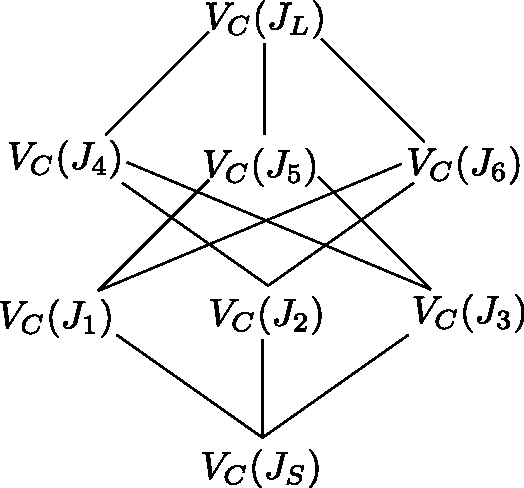
\includegraphics[width=0.8\textwidth]{interpolant_lattice.pdf}
\captionof{figure}{Interpolant lattice}
\label{Fig:int_lat}
% \begin{center}
% \end{figure}
\end{minipage}

It is easy to check  that all $V(J_I)$ satisfy the 3 conditions of
Def. \ref{def:int}. Note also that $V(J_S)$ is the smallest
interpolant, contained in every other interpolant. Likewise, $V(J_L)$
contains all other interpolants and it is the largest. The other
containment relationships are shown in the corresponding interpolant
lattice in Fig. \ref{Fig:int_lat}; i.e. $\Vc(J_1) \subset \Vc(J_5),
\Vc(J_1) \subset \Vc(J_6)$, and so on. 


 %% \begin{align*}
 %% & \Vc(J_1) \subset \Vc(J_5) ~~~~~~~~~~~~ \Vc(J_1) \subset \Vc(J_6) \\
 %% & \Vc(J_2) \subset \Vc(J_4) ~~~~~~~~~~~~ \Vc(J_2) \subset \Vc(J_6) \\
 %% & \Vc(J_3) \subset \Vc(J_4) ~~~~~~~~~~~~ \Vc(J_3) \subset \Vc(J_5)
 %% \end{align*}


}
\end{Example}



%% \begin{Example}
%% \label{example:jajb}
%% Consider the ideal $J_A$ from Example \ref{example:ja} and another
%% $J_B = \langle b,d,ec+e+c+1, ec \rangle$ with the variables of 
%% its generators partitioned as $B = \{e\}$ and $C = \{b,c,d\}$.
%% The intersection of varieties $\Vabc(J_A)$ and $\Vabc(J_B)$ is 
%% empty as,
%% \begin{align*}
%% \Vabc(J_A) &= \Fq^B \times \Vac(J_A)  \\
%% &= (abcde):\{ 01000,00010,01100,10010, \\
%% & ~~~~~~~~~~~~~~~~~~~~~~ 01001,00011,01101,10011 \} \\
%% \Vabc(J_B) &= \Fq^A \times \Vbc(J_B) \\
%% &= (abcde):\{00001,00100,10001,10100\}
%% \end{align*} 

%% Therefore, there must exist an interpolant satisfying the 
%% above three properties. 
%% \end{Example}


\begin{Theorem}
An ideal-interpolant $J_I$, and correspondingly the interpolant $\Vabc(J_I)$, as
given in Def. \ref{def:int}, always exists. 
\end{Theorem}

\begin{proof}
Consider the elimination ideal $J_I = J_A \cap \Fq[C]$. We show $J_I$ satisfies 
the three conditions for the interpolant. 

\par \noindent  \underline{Condition 1}: $\Vabc(J_I) \supseteq
\Vabc(J_A)$. This condition is trivially satisfied due  to
construction of elimination ideals. As $J_I \subseteq J_A$,
$\Vabc(J_I) \supseteq \Vabc(J_A)$.

%% In other words  any point in the $\Vabc(J_A)$ has
%% to satisfy all the polynomials in $J_I$ as $J_I$ is  a subset of
%% polynomials in $J_A$.  

\par \noindent \underline{Condition 2}: $\Vabc(J_I) \cap \Vabc(J_B) =
\emptyset$. This condition  can be equivalently stated as $\Vbc(J_I)
\cap \Vbc(J_B) = \emptyset$ as neither  $J_I$ nor $J_B$ contains any
variables from the set $A$. We prove this condition by
contradiction. Let's assume that there exists a
common point $(\mathbf{b},\mathbf{c})$ in $\Vbc(J_I)$ and $\Vbc(J_B)$.  
We know that the projection of the variety $Pr_A(\Vac(J_A))$ is equal
to the variety of the elimination ideal $\Vc(J_I)$, where $J_I=J_A
\cap \Fq[C]$, due to Lemma \ref{lemma:project}. 
 %% (as $J_A$ is radical). 
Therefore, the point $(\mathbf{c})$ in the variety of $J_I$ can be
extended to a point $(\mathbf{a},\mathbf{c})$ in the variety of
$J_A$. This implies that the ideals $J_A$ and $J_B$ vanish at 
($\mathbf{a},\mathbf{b},\mathbf{c}$). This is a contradiction to our
initial assumption that the intersection of the varieties of $J_A$ and
$J_B$ is empty.  Thus $J_I, J_B$ have no common zeros.

\par \noindent \underline{Condition 3}: The generators of $J_I$
contain only the $C$-variables. This condition is trivially satisfied
as $J_I$ is the elimination ideal obtained by  eliminating
$A$-variables in $J_A$. 
\end{proof}

The above theorem not only proves the existence of an interpolant, but
also gives a procedure to construct one: $J_I = J_A\cap\Fq[C]$. In
other words, compute a reduced Gr\"obner basis $G$ of $J_A$ w.r.t. an
elimination order $A> B > C$ and take $G_I = G \cap \Fq[C]$. Then
$G_I$ gives the generators for the ideal-interpolant $J_I$.

\begin{Example}
{\it 
The elimination ideal $J_I$ computed for $J_A$ from Example \ref{ex:main}
is $J_I = J_S = \langle cd,b+d+1 \rangle$ with variety
$\Vc(J_I)=(bcd):\{001,100,110\}$.  This variety over the variable set
$A$ and $C$ is $\Vac(J_I)=(abcd):\{0001,0100,0110, 1001,1100,1110\}$,
and it contains $\Vac(J_A)$. Moreover, $\Vabc(J_I)$ also has an empty
intersection with $\Vabc(J_B)$. 
}
\end{Example}

%The next theorem proves that this variety $\Vc(J_I)$ is also the
%smallest interpolant, $i.e.$ all other interpolants contain it. 

\begin{Theorem}
\label{thm:smallest}
The interpolant $\Vabc(J_S)$ corresponding to the ideal %-interpolant
$J_S = J_A \cap \Fq[C]$ is the smallest interpolant.
\end{Theorem}

\begin{proof} 
The proof is given in the appendix. 


%% Let $J_I \subseteq \Fq[C]$ be any another ideal-interpolant $\neq
%% J_S$. We show that $\Vc(J_S) \subseteq \Vc(J_I)$. For $\Vc(J_I)$
%% to be an interpolant it must satisfy 
%% \begin{align*}
%% \Vabc(J_A) \subseteq \Vabc(J_I)
%% \end{align*}
%% which is equivalent to 
%% \begin{align*}
%% I(\Vabc(J_A)) &\supseteq I(\Vabc(J_I)) \\
%% \implies J_A &\supseteq J_I  
%% \end{align*}
%% due to Theorem \ref{thm:strong-ns}.
%% %% as $J_I$ is radical so $I(\Vabc(J_I)) = J_I)$. 
%% As the generators of $J_I$ only contain polynomials in $C$-variables,
%% this relation also holds for the following
%% \begin{align*}
%% J_A \cap \Fq[C] &\supseteq J_I \\
%% \implies J_S &\supseteq J_I \\
%% \implies \Vc(J_S) &\subseteq \Vc(J_I).
%% \end{align*} 
\end{proof}

%After proving that the elimination ideal $J_A \cap \Fq[C]$ is the
%smallest interpolant, 
Now we discuss how the largest interpolant can be
computed. For this, we will make use of quotients of ideals. 

\begin{Definition}
\label{def:quo}
({Quotient of Ideals}) If $J_1$ and $J_2$ are ideals in a ring $R$,
then $J_1:J_2$ is the set 
%  \begin{equation}
  $\{f \in R \ |\ f\cdot g \in J_1, \forall g \in J_2\}$ %\nonumber
%  \end{equation}
and is called the {\bf ideal quotient} of $J_1$ by $J_2$.
\end{Definition}

We use ideal quotients to compute the complement of a variety. Given
an ideal $J' \subset R$ containing the vanishing polynomials, suppose
we need to find an ideal $J$ such that $V(J) = \Fq^n - V(J') = V(J_0)
- V(J')$, where ``$-$'' corresponds to the set difference
operation. Then $J = J_0 : J'$ (see Theorem III.2 and Corollary III.1
in \cite{xiaojun:hldvt2016} for a proof outline). Once again, the
Gr\"obner basis algorithm can be used to compute $J_0:J'$ 
\cite{ideals:book}.  

\begin{Theorem}
\label{thm:large}
Consider the elimination ideal $J'_L = J_B \cap \Fq[C]$. The
complement of the variety $\Vc(J'_L)$,  computed as $\Fq^C - \Vc(J'_L)$,
is the largest interpolant.
\end{Theorem}

\begin{proof} Proof is given in the appendix. 

%% We first prove that the interpolant computed by
%% complementing $\Vc(J'_L)$  as $\Fq^C - \Vc(J'_L)$ is indeed a valid
%% interpolant. As $J'_L$ is the elimination ideal computed from $J_B$,
%% $\Vbc(J'_L) \supseteq \Vbc(J_B)$. This in turn implies that the
%% complement of $V(J'_L)$ cannot intersect with $V(J_B)$ at any
%% point. This proves condition 2 for $\Fq^C - \Vc(J'_L)$ to be a
%% valid interpolant.  

%% For condition 1, we need to prove that
%% \begin{align*}
%% \Vac(J_A) \subseteq \Fq^A \times (\Fq^C - \Vc(J'_L))
%% \end{align*}
%% This can be restated as
%% \begin{align*}
%% \Vac(J_A) \cap \Fq^A \times \Vc(J'_L) = \emptyset
%% \end{align*}
%% Let us assume (by contradiction) that there exists a common point 
%% $(\mathbf{a},\mathbf{c})$ in $\Vac(J_A)$ and $\Fq^A \times
%% V_C(J'_L)$. As the projection $Pr_B(\Vbc(J_B))$ on the
%% $C$-variables is equal to  the variety of the elimination ideal
%% $\Vc(J'_L)$, a point $(\mathbf{c}) \in \Vc(J'_L)$ can be  extended to
%% some point $(\mathbf{b},\mathbf{c})$ in $\Vbc(J_B)$. This implies that
%% the point $(\mathbf{a},\mathbf{b},\mathbf{c})$ is a common point in
%% $\Vabc(J_A)$ and $\Vabc(J_B)$, which is a contradiction to our initial
%% assumption. Therefore condition 1 of Def. \ref{def:int} is satisfied
%% too and $\Fq^C - \Vc(J'_L)$ is indeed an interpolant. 

%% \par \noindent Next we prove that $\Fq^C - \Vc(J'_L)$ is the largest
%% interpolant. Consider an arbitrary ideal-interpolant $J_I$. We want to
%% prove $\Vc(J_I) \subseteq \Fq^C - \Vc(J'_L)$, or equivalently to prove
%% $\Vc(J_I) \cap \Vc(J'_L) = \emptyset$. Let us assume (by contradiction) 
%% that there exists a common point $(\mathbf{c})$ in $\Vc(J_I)$ and
%% $\Vc(J'_L)$. As $J'_L$ is the elimination ideal of $J_B$, this point
%% can be extended to some point $(\mathbf{b},\mathbf{c})$  
%% in $\Vbc(J_B)$. This in turn implies that $(\mathbf{b},\mathbf{c})$ is
%% a common point in  $\Vbc(J_B)$ and $\Fq^B \times \Vc(J_I)$. This is a
%% contradiction as an interpolant cannot intersect with the variety of
%% $J_B$. Hence, $\Fq^C - \Vc(J'_L)$ is the largest interpolant and it
%% contains all other interpolants.

\end{proof}

Let $J_L$ be the radical ideal corresponding to the largest
interpolant $\Vc(J_L) = \Fq^C - \Vc(J'_L)$. This ideal-interpolant
$J_L$ can be computed as $J_L = (J_{0,C}:J'_L)$, where $J_{0,C}$ is
ideal of vanishing polynomials in $C$-variables.  


\begin{Example}
{\it 
The ideal-interpolant $J_L = \langle bd + b + d + 1 \rangle$ in 
Example~\ref{ex:main} is computed as:
\begin{itemize}
	\item First compute the ideal $J'_L = J_B \cap \Fq[C]$ which results in 
	$J'_L = \langle b,d \rangle$.
	\item Then compute $J_L$ as $J_L = J_{0,C}: J'_L$ which results in
	$J_L = \langle bd + b + d + 1 \rangle$
\end{itemize}
The variety $V_C(J_L)=(bcd):\{001,011,100,101,110,111\}$ and it is the
largest interpolant for the given pair ($J_A,J_B$). 
}
\end{Example}

\begin{Lemma}
\label{noofinter}
The total number of interpolants for the pair ($J_A,J_B$) is
$2^{|SM(J_D)|}$, where $J_D = (J_L:J_S)$. 
\end{Lemma}

\begin{proof}
The proof is given in the appendix. 

%% The smallest and the largest interpolants are $\Vc(J_S)$ and $\Vc(J_L)$,
%% respectively. The set difference $\Vc(J_L) - \Vc(J_S)$ is also a
%% variety of some ideal $J_D$, which can be computed as
%% $J_D=(J_L:J_S)$. By selecting different subsets of $\Vc(J_D)$ and
%% adding them to $\Vc(J_S)$, we can generate all the 
%% interpolants. Consider, 
%% \begin{align*}
%% \label{eqn:pwsetjd}
%% \binom{|\Vc(J_D)|}{0} + \binom{|\Vc(J_D)|}{1} + \cdots + \binom{|\Vc(J_D)|}{|\Vc(J_D)|} = 2^{|\Vc(J_D)|}
%% \end{align*}
%% where the term $\binom{|\Vc(J_D)|}{0}$ denotes that no point is selected from $\Vc(J_D)$ and results in 
%% $\Vc(J_S)$ as the ideal-interpolant. On the other hand, the term $\binom{|\Vc(J_D)|}{|\Vc(J_D)|}$ is equivalent 
%% to selecting  all the points from $\Vc(J_D)$ and results in $J_L$ as 
%% the ideal-interpolant. So the number of interpolants is equal to
%% $2^{|\Vc(J_D)|}$. Theorem \ref{thm:count} further tells us that the 
%% cardinality of a variety of an ideal is equal to the number of
%% standard monomials of that ideal, therefore, number of interpolants $=
%% 2^{|SM(J_D)|}$.  

\end{proof}

\begin{Example}
\label{ex:jd}
{\it 
From Example~\ref{ex:main}
$J_L = \langle bd + b + d + 1 \rangle$ and $J_S = \langle cd, b + d+
1\rangle$. 
Computing $J_D = J_L : J_S$ gives $J_D = \langle
d+1,bc+b+c+1,c^2+c,b^2+b \rangle$, where the variety $\Vc(J_D)=\Vc(J_L)-\Vc(J_S)
=(bcd):\{011,101,111\}$. 

The standard monomials for $J_D$ are $SM(J_D) = \{1,b,c\}$. Therefore,
the total number of interpolants for the given pair ($J_A,J_B$) is
$2^{|\{1,b,c\}|}=2^3=8$. 
}
\end{Example}


\subsubsection{The structure of the interpolant lattice:} Note that
our results do provide some insights into the structure of the
interpolant lattice. Let $l = |SM(J_D)|$. Then, the height of the
interpolant lattice is $l + 1$, and the number of elements (interpolants) at each
level $i$ is $l \choose i$, $0\leq i \leq l$. Notice also that the size (height and
width) of the interpolant lattice is independent of the number of
variables in the set $C$, and depends only on $|SM(J_D)|$. 

%% Next we describe a procedure for enumerating all of these interpolants using the $SM(J_D)$.
%% Let's say there are $l$ standard monomials, $\{m_1,\dots,m_l\}$ in the set $SM(J_D)$. Consider
%% a polynomial $f_i$ constructed using the linear combination of $\{m_1,\dots,m_l\}$ as,
%% \begin{center}
%% $f_i = \lambda_1\cdot m_1 + \lambda_2\cdot m_2 +\cdots+ \lambda_l\cdot m_l$
%% \end{center} 
%% where each $\lambda_i \in \mathbb{F}_2$ $i.e.$ $\lambda_i \in \{0,1\}$.
%% There can be exactly $2^l$ unique polynomials obtained in this way.
%% We can then obtain all the ideal-interpolants $I_j$ as,
%% \begin{center}
%% $I_j = J_S\cdot(J_D + \langle f_i \rangle)$
%% \end{center}
%% where $\langle f_i \rangle$ is the ideal generated by the polynomial $f_i$.
